%%%%%%%%%%%%%%%%%%%%%%%%%%%%%%%%%%%%%%%%%%%%%%%%%%%%%%%%%%%%%%%%%%%%%%%%%%%
% sample.tex
%   - Originally written by hyuga.
% これはサンプル記事です。
% この記事をコピーして、思いの丈を書き綴ってください。
% また、この記事は解説にもなっているので、執筆前に一読しましょう。
%%%%%%%%%%%%%%%%%%%%%%%%%%%%%%%%%%%%%%%%%%%%%%%%%%%%%%%%%%%%%%%%%%%%%%%%%%%

% ソースコードを記事内に入れたい場合には、
% \inputsource[caption=キャプション,label=ラベル]{言語名}{ソースコードファイル名}
% で出力できます。

% 記事のタイトルや著者を指定します。
% \genkoutitle{記事のタイトル}{記事のサブタイトル}{著者名}{著者エイリアス}{部門名(現在使用不可)}
\genkoutitle{Androidのゲームアプリをリリースしました}{}{momasahiro}{}{}

%%%%%%%%%%%%%%%%%%%%%%%%%%%%%%%%%%%%%%%%%%%%%%%%%%%%%%%%%%%%%%%%%%%%%%%%%%%
% 記事を書く場合は、これ以下のテキストをひと思いに削除しちゃってください。
% なお、本文で使える見出し出力コマンドは \section 以下です。
%%%%%%%%%%%%%%%%%%%%%%%%%%%%%%%%%%%%%%%%%%%%%%%%%%%%%%%%%%%%%%%%%%%%%%%%%%%

\section{はじめに}
タイトル通りですが、2週間ほど前にアプリをリリースしました。
内容は簡単なパズル的なミニゲームです。
普段は脱出ゲームを作ることが多いですが、ミニゲームの場合どのくらいダウンロードされるのかなどを知りたかったこともあり今回は違うジャンルのものを開発しました。

\section{ゲーム内容}
タイトルは「Primes」です。詳しいルールは省略しますが、簡単に言うと、数字の書かれたタイルを動かして
\begin{itemize}
	\item 素数のタイルのみ動かせる
	\item 素数でないタイルは分裂する
\end{itemize}
という条件で大きな数を育てていくようなゲームです。
\begin{center}
	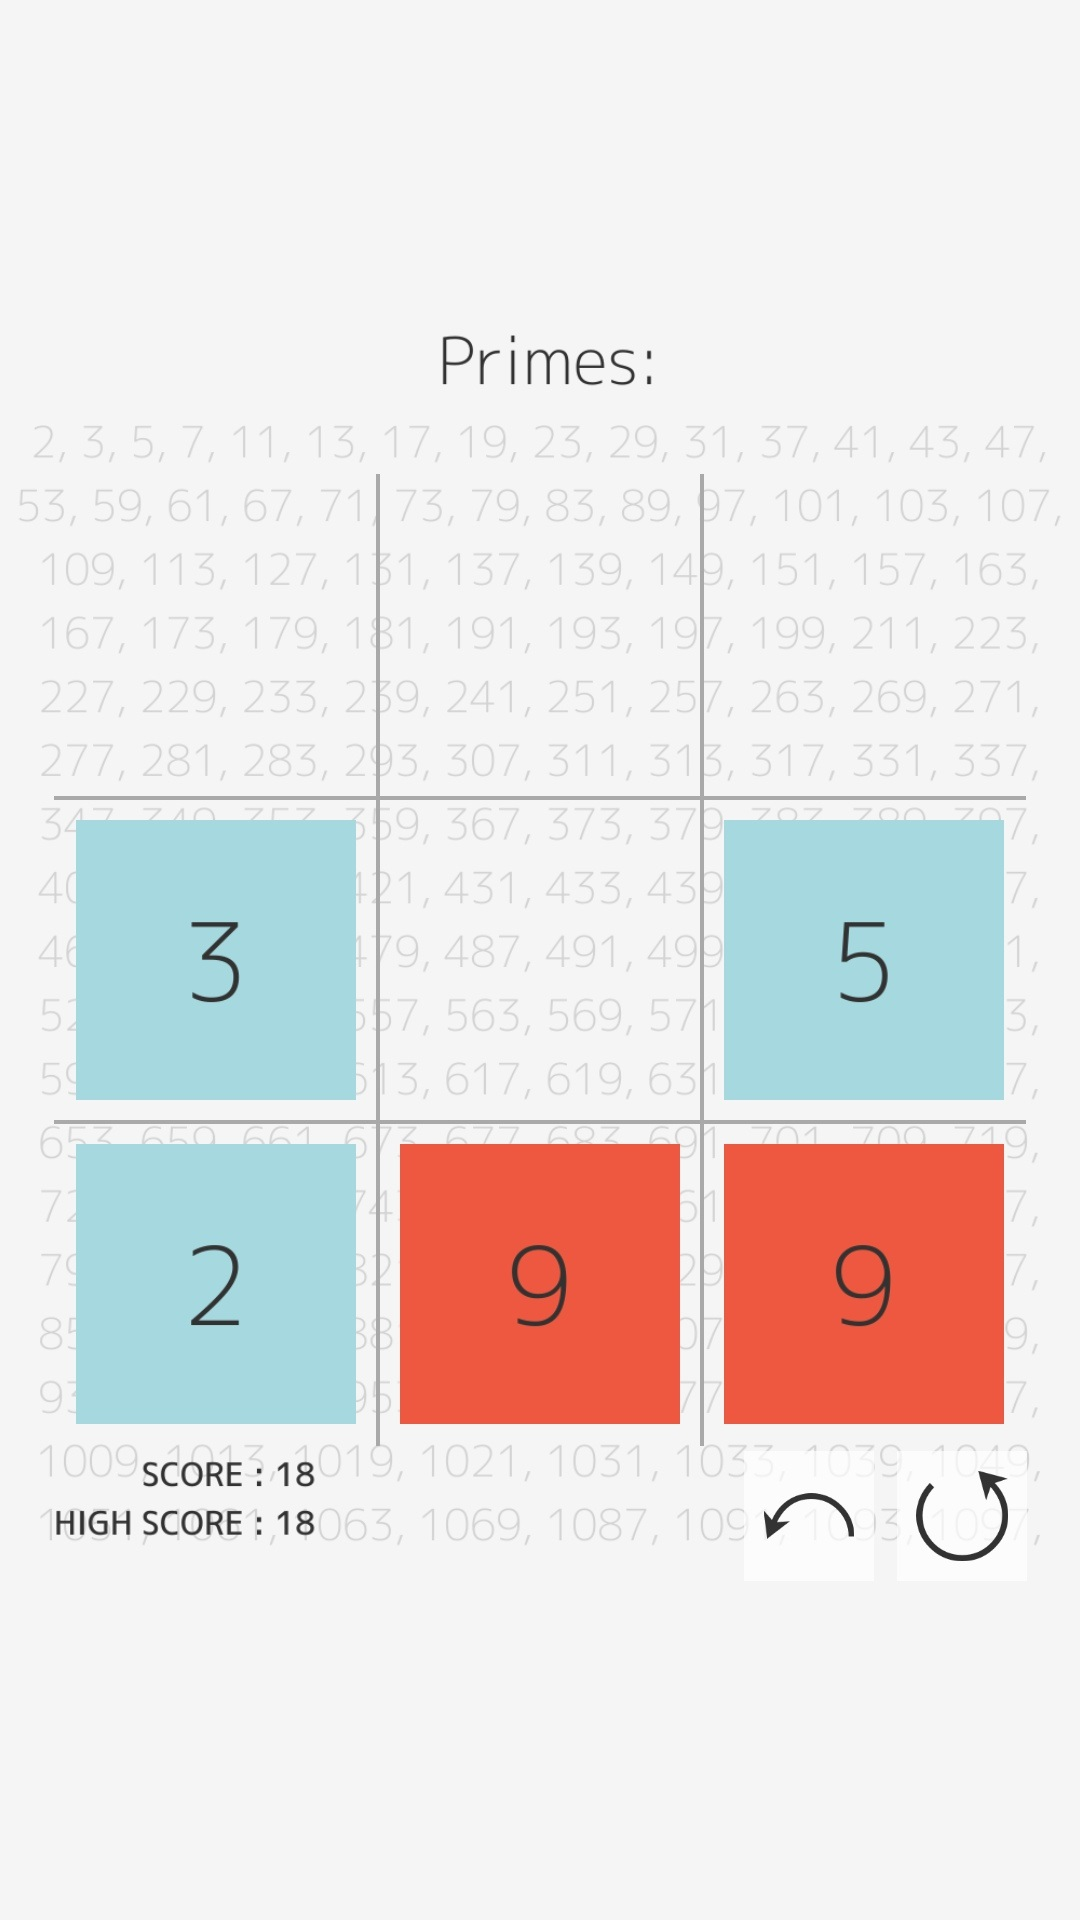
\includegraphics[width=4cm]{screen1.jpg}
	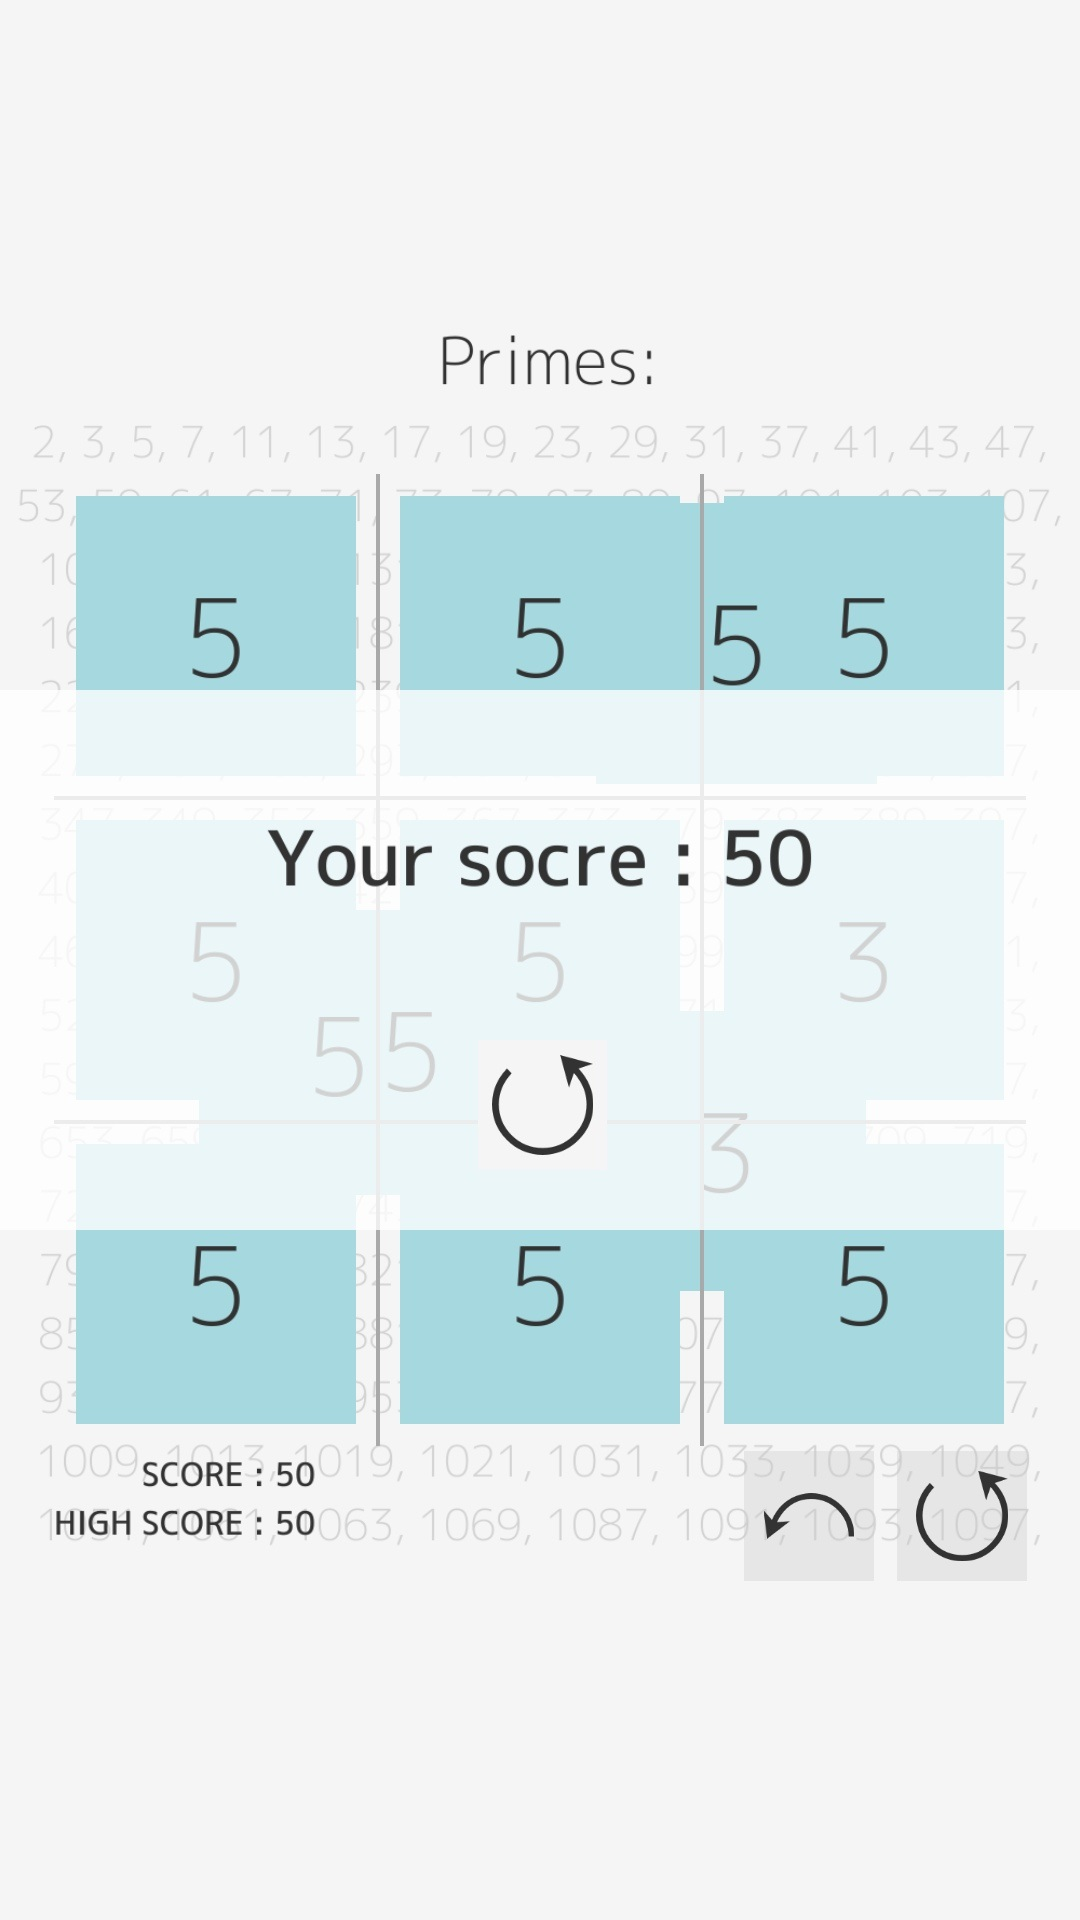
\includegraphics[width=4cm]{screen2.jpg}
\end{center}
\section{リリース後}
あまりダウンロード数が伸びません。
脱出ゲームの場合はブラウザ版も公開していて、個人開発でも脱出ゲームを紹介してくださるサイトは多数存在し、そこからの流入で結構ダウンロードしてもらえますが、ミニゲームの場合はそうはいかないようです。
今回のゲームも一応ブラウザ版も公開していますが、ブラウザのミニゲームを紹介しているサイトはあまり無い感じでした。
とはいえ、ミニゲームは開発が簡単で作業量も少なく開発できるので、これからも何か思いついたら作りたいと思いました。

\section{おわりに}
Primesは、GooglePlayからダウンロードできます。
\begin{center}
	
\includegraphics[width=4cm]{qr.png}
\end{center}
\begin{center}
	https://play.google.com/store/apps/details?id=com.masasgames.Primes
\end{center}

Androidを持っている方でプレイしたいという方がいらっしゃれば、是非プレイしてみてください。